\subsection{Impacts of prediction errors}
\label{sec:ImpactOfPredictionErrors}

%Since the capacity planning of a data center is executed in the long-run, it suffers from prediction errors.

%To study the impact prediction errors on capacity planning
Prediction errors are generally negligible during operational management, which happens in real-time. Hence, GRID and DEM are not affected by the prediction errors because they do not need capacity planning. On the other hand, SUP and PROP suffer from prediction errors because they provide the capacity planning decisions, and then operate the data center in real-time based on the planned capacities. We normalize the root mean squared errors (RMSE) compared to the means of interactive workloads, batch jobs, capacity factors of PV, electricity prices, and gas prices, respectively. For instance, when normalized RMSEs are $0.2$, the RMSEs of all the aforementioned predictions are 20\% of their means. 

Figure {\ref{f.cost_err_comparison}} shows the impacts of prediction errors on the total expenditures of the four methods. As the prediction errors become large (more than 10\%), the total costs of SUP and PRO go up while the costs of GRID and DEM stay unchanged. Interestingly, total cost of the proposed framework is still the best and achieves the significant cost savings, i.e., 58\% of GRID. The intuition behind this is that the operational management is cost-efficient in using the various power sources and scheduling the batch jobs to compensate for the prediction errors.

The impacts of prediction errors on emissions are presented in Figure {\ref{f.emission_err_comparison}}. As the prediction errors increase, the emissions of PROP go up. However, PROP still reduces 49\% of emissions reduction compared to GRID. Specially, the emissions stay unchanged when RMSE is greater than 0.2.
%The curve of the supply-only method is more interesting. It first does not change much at normalized errors less than $0.05$, goes up from $0.05$ to $0.25$, and finally goes down as the normalized errors greater than $0.25$. Because of prediction errors, the supply-only method over-provisions the PV capacity. When the prediction errors are too small, the over-provisioned PV capacity is useful in reducing the emissions. When the normalized errors become larger, the supply-only method uses more electricity grid to compensate the renewable energy which causes more emissions. However, when the electricity prices are very unpredictable, it prefers the gas engines that release less emissions than the public electricity grid.

\hideit{
\begin{figure}[!th]
	\vspace{-0.1cm}
 \begin{center} 
 \subfigure[Expenditures]{{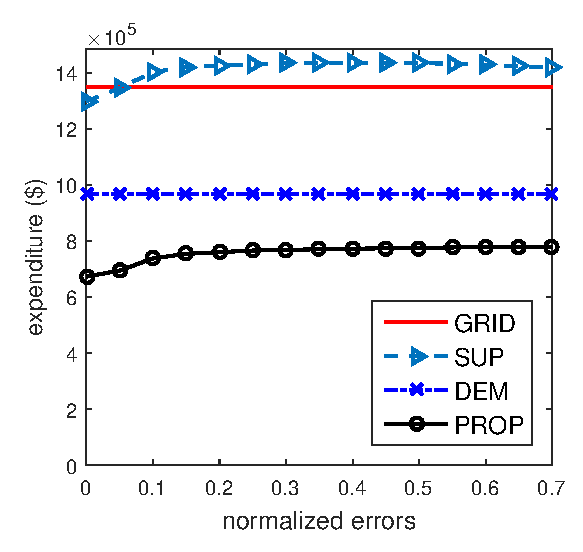
\includegraphics[width=0.32\columnwidth]{figs/cost_err_comparison}}
 \label{f.cost_err_comparison}} 
 \subfigure[Emissions]{{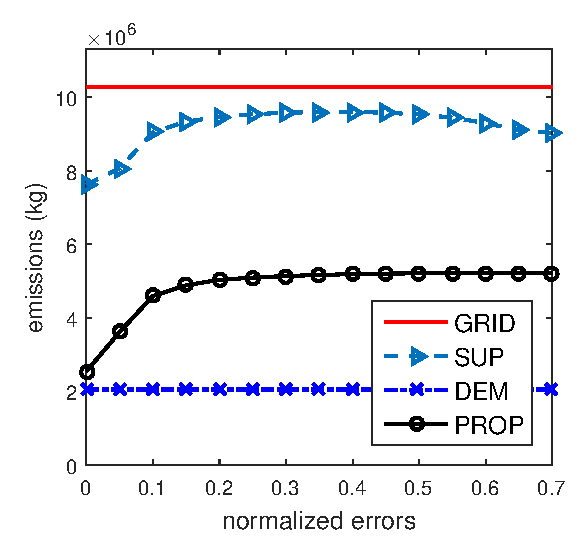
\includegraphics[width=0.32\columnwidth]{figs/emission_err_comparison}}
 \label{f.emission_err_comparison}} 
 \caption{Impacts of prediction errors. Under large prediction errors, the proposed framework still achieves the significant cost and emission reductions.} 
 \label{f.prediction}
 \end{center}
  \vspace{-0.3cm}
\end{figure}
}
\textbf{\textit{Key insights}}: Under large prediction errors, our proposed framework still achieves significant cost and emission reductions compared to the baseline methods.